\setchapterimage[8.5cm]{tde}
\setchapterpreamble[u]{\margintoc}
\chapter{Stacking Analyses with IceCube}
\labch{results}
\begin{fquote}[Ronald Fischer][The Design of Experiments][1935]Every experiment may be said to exist only in order to give the facts a chance of disproving the null hypothesis.
\end{fquote}


What did we see? Excellent question...

\section{TDEs}

As part of this thesis, a stacking analysis was performed searching for neutrino emission from Tidal Disruption Events (see Chapter \ref{ch:sources}). This was the first experimental search for such a correlation. The search was performed using the \emph{\href{https://github.com/IceCubeOpenSource/flarestack}{Flarestack}} code introduced in Chapter \ref{ch:llh}.

\subsection{Neutrino Production Scenarios in TDEs}

As outlined Chapter \ref{ch:sources}, theoretical modelling of neutrino emission in TDEs generally distinguish between those with relativistic jets and those without. In recognition of this, we ultimately have two distinct hypotheses to test:

\begin{itemize}
	\item Neutrino emission in on-axis jetted TDEs
	\item Neutrino emission in "non-jetted" TDEs
\end{itemize}

In general, the timescales predicted for neutrino emission have varied substantially. In general, neutrino emission is expected to occur close to the peak EM brightness of the flare, with durations of a few hours to $\sim$ 100 days. There are no scenarios for neutrino emission preceding disruption. 

\subsection{TDE Catalogues}

To perform a correlation analysis, a source list must first be compiled to test. A catalogue of TDEs is maintained by the \emph{\href{https://tde.space/}{OpenTDECatalog}} \sidecite{tde_catalog_paper}, containing relevant metadata and photometry. The database prioritises completeness by containing all objects with a possible TDE classification, even if this is not a secure classification \cite{tde_catalog_paper}, and will thus by construction suffer from source contamination. The database itself is maintained by volunteers, and is thus not entirely complete. For the compilation of a catalogue for this thesis, the list from the \emph{\href{https://tde.space/}{OpenTDECatalog}} was supplemented by additional objects and data from the literature.

At the time of catalogue compilation in 2018, this database contained approximately 70 objects. Of these, 3 had clear evidence of on-axis relativistic jets, while the remaining 67 did not. We further exclude those objects with peaks >100 days before the start of data-taking during the IC40 data season on 4th May 2008 (see Chapter \ref{ch:icecube}), as these objects do not overlap our neutrino dataset. We are left with 53 TDEs for correlation.

From the starting point of all TDEs, one distinct subsample was created:

\begin{itemize}
	\item \textbf{Jetted TDEs} are X-Ray-bright TDEs which launched relativistic jets pointing towards the Earth. There are three jetted TDEs, and neutrino emission is most promising from this category
\end{itemize}

These three Jetted TDEs share similar properties, namely that they were all sufficiently bright to be discovered by the \textit{Swift}-BAT X-ray telescope. They each have well-sampled lightcurves, with the time of jet-launching constrained to a window of a few days. Given the consistent observational features of luminous, hard X-ray emission which rapidly fades, it is likely that all three objects are indeed jetted TDEs.

On the other hand, the properties of the non-jetted TDEs are highly heterogeneous, discovered across a range of wavelengths (e.g X-ray, Optical, IR) with varying multi-wavelength coverage. There are a handful of compelling TDE candidates, primarily those with comprehensive multi-epoch spectroscopic observations, for which alternative explanations are disfavoured. To avoid catalogue contamination of by missclassified AGN or SN, we define a clean "golden sample" consisting of these reliably-classified TDEs:

\begin{itemize}
	\item \textbf{Golden TDEs} are strong candidates where the TDE interpretation is supported by multiple spectra
\end{itemize}

Of the remaining TDE candidates, there is one distinct subclass of coherent flares observed in dusty galaxies via IR emission \sidecite{wang_mir_tdes_2018}. The rate of decay in those galaxies is consistent with the evolution expected for a TDE. However, we would then expect these galaxies contain TDEs which are obscured by dust, with this dust then slowly reprocessing the EM flare in the galaxy core.  For such reprocessing, there would likely be a variable time lag between the disruption itself and the corresponding IR flare. As we expect that neutrinos should generally arrive after the disruption, these timescales for neutrino emission from obscured TDEs has significant additional uncertainty. 

We treat these obscuted TDEs separately from the other "silver sample" TDEs:

\begin{itemize}
		\item \textbf{Obscured TDEs} are TDE candidates which occur in very dusty galaxies, and are only observed via reprocessed infra-red emission. 
	\item \textbf{Silver TDEs} are all other candidates, where a TDE interpretation is either likely or not disfavoured.
\end{itemize}

These catalogues are summarised in Table \ref{tab:stacking_cat}.

\begin{table*}[]
	\centering
	\begin{tabular}{||c c c c |} 
		\hline
		Catalogue & Source Class & Size & Description \\ [0.5ex] 
		\hline\hline
		Jetted & Jetted TDEs &  3 & \textit{Probable TDEs with on-axis jets}\\ 
		\hline
		Golden & Non-Jetted TDEs & 13 & \textit{Probable TDEs with convincing classification}\\
		\hline
		Silver & Non-Jetted TDEs & 24 & \textit{Candidate TDEs with ambiguous classification}\\
		\hline
		Obscured & Non-Jetted TDEs & 13 & \textit{Candidate TDEs in dusty galaxies}\\[1ex] 
		\hline
	\end{tabular}
	\caption{Summary of the four TDE catalogues..}
	\label{tab:stacking_cat}
\end{table*}{}

\subsection{Search Windows}

To account for the heterogeneous datasets, an individual search window was defined for each TDE. For jetted/gold/silver TDE, the following criteria were used:

\begin{itemize}
	\item For TDEs in which the light curve was observed when rising, the first measurement is taken as the window start.
	
	\item For TDEs without an observation during lightcurve rise, the last upper limit is taken as the window start.
	
	\item The maximum date was taken as the date on which the brightest TDE luminosity measurement was performed.
	
	\item The window extends from the defined window start to 100 days after the maximum date
	
\end{itemize}

Applying these criteria gives a tailored search window for each TDE. To account for potential delay following neutrino emission, Obscured TDEs instead had a search window extending from 300 days before peak to 100 days after peak. The four catalogues, including search windows, are provided in the Appendix. It is the first such catalogue to contain time windows, and could be used for stacking analyses of e.g gamma-ray emission.

\subsection{Likelihood Analysis and Results}

As outlined in Chapter \ref{ch:llh}, a stacking analysis requires an additional statement on the expected relative neutrino emission of each source in a catalogue. However, these TDE catalogues are characterised by small numbers of heterogeneous sources. With a mix of multi-wavelength coverage and cadences, there is no obvious proxy for neutrino emission. A common standard-candle approximation, in which each source has the same intrinsic luminosity, is also not well-motivated. There is no evidence of standard-candle behaviour in EM wavelengths, so there is no reason to think it would hold for neutrino emission. We are left with no clear method to compare the relative contributions, and for this reason, an agnostic approach is applied. Using the method outlined in Section \ref{sec:fit_weights}, we fit the contribution of each source in the catalogue individually, requiring only that they share a common neutrino spectrum.

Following the procedure in Chapter \ref{ch:llh}, we perform an unbinned likelihood analysis to obtain results for each catalogue, with fit parameters TS, $\gamma$ and a number of signal events for each source ($n_{k}$). We also obtain a final Test Statistic (TS) value, and calculate a p-value for this TS using pseudotrials. Table \ref{tab:stacking_tests} summarises the results for each catalogue, including $n_{s} = \sum n_{k}$. The individual $n_{k}$ values are provided in the Appendix Chapter \ref{ch:catalogues}.

\begin{table*}[]
	\centering
	\begin{tabular}{||c c c| c c c | c||} 
		\hline
		Catalogue & Source Class & Size & $n_{s}$  & $\gamma$ & TS & Pre-trial p-value\\ [0.5ex] 
		\hline\hline
		Jetted & Jetted TDEs &  3 & 1.5& 4.0&0.77&0.40\\ 
		\hline
		Golden & Non-Jetted TDEs & 13 &3.9&2.4& 2.4&???1.0\\
		\hline
		Silver & Non-Jetted TDEs & 24 &15.6&2.7&7.79& ???1.0\\
		\hline
		Obscured & Non-Jetted TDEs & 13 &29.4&2.8&14.7&???\\[1ex] 
		\hline
	\end{tabular}
	\caption{Summary of the results for the four TDE catalogues. For each, an independent stacking analysis was performed. The catalogues covered sources from May 2008 to October 2017, matching the IceCube data-taking period.}
	\label{tab:stacking_tests}
\end{table*}{}

There was no significant correlation identified for any of the catalogues. While the Obscured TDE catalogue yielded the most significant pre-trial p-value, after trial correction using Equation \ref{eq:trial_correction} this reduces to $p_{\textup{post-trial}}$=0.25, and is thus entirely consistent with background expectations. No discovery of neutrino emission from TDEs is claimed, and \emph{we do not reject the null hypothesis that TDEs and neutrinos are uncorrelated}.

\subsection{Limits on catalogue neutrino emission}

Being unable to reject the null hypothesis, we can instead set an upper limit on neutrino emission, by ruling out scenarios for which we would have expected to reject the null hypothesis. We follow the procedure outlined in Section \ref{sec:sens_uls} to set an upper limit, at 90\% confidence, using pseudoexperiements with simulated signal. These limits are only valid \emph{under the assumption that the signal looks like the baseline IceCube MC}, and thus that \emph{the impact of all systematic effects are negligible}.

While our search results in Table \ref{tab:stacking_tests} are agnostic to the relative neutrino contribution of each source, any pseudoexperiments involving simulated signal must make an assumption regarding the intrinsic neutrino luminosity of each source. Though it remains a poor approximation for EM emission, we inject neutrinos under \emph{the assumption that each catalogue source emits the same intrinsic energy in neutrinos}. The corresponding flux on Earth is thus proportional to the inverse distance squared of each source. This flux is injected uniformly across the search windows for each source, as defined in Appendix X. To conserve energy, and the flux-per-source is then inversely proportional to the length of the search window. The intrinsic energies are presented as \emph{isotropic-equivalent}, and thus quoted assuming that the emission is emitted isotropically. This is of particular relevance for the Jetted TDEs, for which emission is likely to be highly beamed, and the energy would then be scaled accordingly. All limits derived below are only valid in the case that all of these assumptions are true.

Upper limits are derived under the \emph{assumption of an unbroken neutrino power law, between 100 GeV and 10 PeV}, for a variety of spectral limits. These upper limits are shown in Figure \ref{fig:cat_upper_limit}, for both the catalogue fluence (left y axis) and the corresponding energy per source (right y axis). 

\begin{figure}[!ht]
	\centering 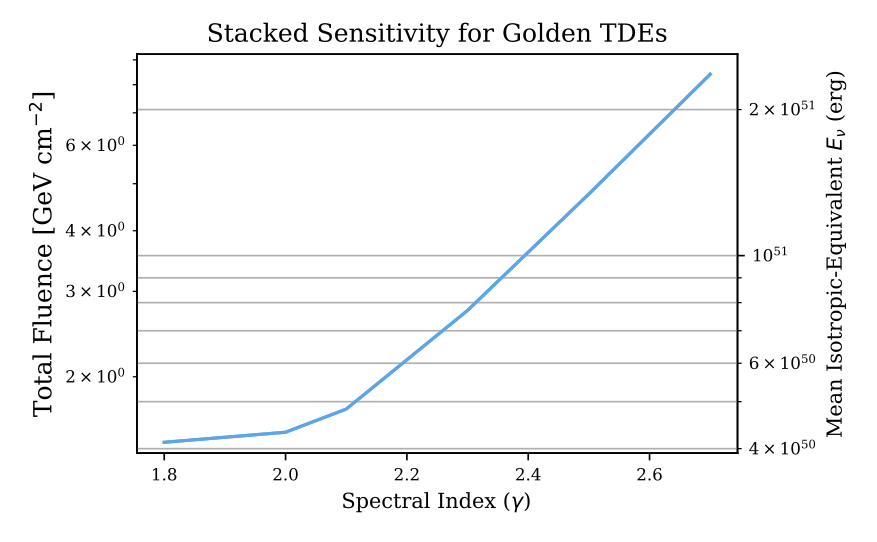
\includegraphics{results/gold_flux}
	\caption{Limits on the neutrino fluence and source energy for each catalogue. (Include numu + numubar in plot)}
	\label{fig:cat_upper_limit}
\end{figure}

Systematics 10\%

\subsection{Limits on population neutrino emission}

While the limits presented above constrain the contribution of those catalogues tested, we ultimately wish to constrain neutrino emission for the TDE population as a whole. If we \emph{assume that catalogue sources are representative of the broader population}, we can extrapolate from our per-source standard candle limits in Figure \ref{fig:cat_upper_limit} to the population flux. We seek to constrain the flux of two populations, namely jetted and non-jetted TDEs. For the latter case, we rely on the results of the golden TDE catalogue, since the extrapolation \emph{implicitly requires that the catalogues are not contaminated by misclassified objects}.

We must multiply the energy-per-source by the rate of TDEs as a function of redshift, yielding an energy-per-redshift-shell. We can then scale with the luminosity distance to derive the flux-per-shell at Earth. By numerically integrating the flux contributed by shells of increasing redshift up to a horizon of z=8, we thus calculate the cumulative flux expected for each population. This method thus accounts for TDEs that were not detected by other surveys, and were therefore not incorporated into our catalogue. 

There a number of subtleties to this method. The rate is given per unit time, but the impact of time dilation at higher redshifts suppresses the rate by a factor (1+z). Furthermore, in much the same way as for photons, neutrinos from distant shells will be "red-shifted" to lower energies. At Earth, for energy $E_{\textup{obs}}$, we will observe neutrinos that were emitted at $E_{\textup{em}} = (1+z) E_{\textup{obs}}$. Thus, for a power law of E$^{-\gamma}$, the flux at $E_{\textup{obs}}$ will be suppressed by a factor of $(1+z) ^{\gamma}$. Both effects are generally small for the sources in the catalogue, because it primarily probes the local universe, but must be accounted for when extrapolating.

To perform this calculation, we use per-source limits for the most recent IceCube global fit of the astrophysical neutrino flux, with a best-fit spectrum of $E^{-2.50}$. For non-jetted TDEs, we assume a central local rate of $8 \times 10^{-7}$ Mpc$^{-3}$ year$^{-1}$ \sidecite{2018ApJ...852...72V}, a source evolution derived by \cite{Sun:2015bda}, and constrain the contribution of TDEs to be less than 26\% of the total. For jetted TDEs, under the assumption that they follow the same underlying source evolution as non-jetted TDEs with a central rate of $3 \times 10^{-11}$ Mpc$^{-3}$ year$^{-1}$ \sidecite{Sun:2015bda}, we find that they must contribute less than 1\% of the total.  These constraints are illustrated in Figure \ref{fig:DiffuseFlux}.

\begin{figure}[!ht]
	\centering 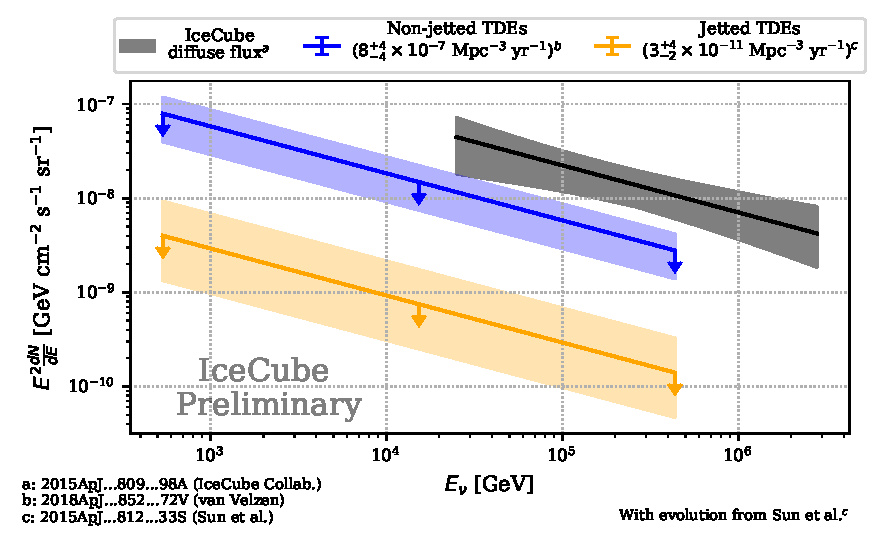
\includegraphics{results/tde_limits}
	\caption{Limits on the contribution of jetted and non-jetted TDEs to the diffuse neutrino flux.}
	\label{fig:DiffuseFlux}
\end{figure}

As the contribution from a population is directly proportional to the local population rate, the shaded bands indicate the uncertainty in our limits arising from rate estimates. For TDEs, these rates are the dominant source of uncertainty in neutrino flux. It will require systematic evaluation of observed TDE rates to enable more precise limits on neutrino emission. Any refined rate estimate can be used to linearly rescale these limits. Propagating through the current local rate uncertainty, we constrain non-jetted TDEs to be less than 13-39\%, and jetted TDEs to be less than 0.n-1.n\% of the total. With a more precise future measurement of the local TDE rate, these values can be linearly rescaled to provide more accurate limits.

Such limits also critically depend on the source evolution of TDEs as a function of redshift, but this is essentially unconstrained observationally because TDEs detections are overwhelmingly confined to the local universe (z $\lesssim$ 0.3). Estimates are made primarily based on theoretical predictions derived from the rate of SuperMassive Black Holes (SMBHs)?? \cite{Sun:2015bda}. If we instead consider a source evolution similar to the Star Formation Rate (SFR), as derived by CLASH-CANDELs, we would find limits of x and y \% respectively. For such a scenario, the contribution of unresolved TDEs is so large that the measured flux itself provides a stricter constraint than the catalogue test?

\subsection{Neutrino Emission from Individual TDEs}

In addition, four TDEs were selected for individual analysis. Two of the three jetted TDEs, Swift J1644+57 and Swift J2058+05, were chosen due to their luminosity, as well as their position in the northern hemisphere where IceCube has the highest effective area. In addition, ASSASN-14li and  XMMSL1 J0740-85 were chosen as non-jetted TDEs which were both nearby and bright. These four TDEs were the only catalogue sources that were also detected in radio observations, typically a tracer for relativistic particle acceleration.

For each of the four individual TDEs, searches were conducted for neutrino clustering in both time and space, following the procedure outlined in Section  \ref{sec:cluster_algorithm}. All single-object tests are described in Table \ref{tab:single_tests}

\begin{table*}[]
	\centering
	\begin{tabular}{||c c c| c |} 
		\hline
		Object & Stacking Catalogue &  Isotropic-Equivalent Energy (ergs) & Pre-trial p-value\\ [0.5ex] 
		\hline\hline
		Swift J1655+57 & Jetted TDEs & $<2 \times 10^{54}$ & 1.0\\ 
		\hline
		Swift J2058+05 & Jetted TDEs & $<2 \times 10^{51}$& 0.38\\
		\hline
		ASASSN-14li & Non-jetted TDEs (Gold) & $<2 \times 10^{51}$& 1.0\\
		\hline
		XMMSL1 J0740-85 & Non-jetted TDEs (Gold)& $<2 \times 10^{51}$ & 0.22\\
		\hline
		\hline
		AT2018cow & - & $<2 \times 10^{51}$& ??\\
		[1ex] 
		\hline
	\end{tabular}
	\caption{Summary of the five individual TDEs for which the temporal-cluster-search method was applied. All but AT2018cow were included in the stacking analysis.}
	\label{tab:single_tests}
\end{table*}{}

\section{AT2018cow and FBOTs}

Following the four stacking analyses and four object analyses described in Chapter \ref{ch:llh}, an additional analysis was performed on AT2018cow. This object was a fast, bright, blue transient first discovered in 2018 cite. The observations suggested AT2018cow was a nearby example of a recently-identified population of Fast Blue Optical Transients (FBOTs) \sidecite{Margutti:2018rri}. 

Shortly after the time of discovery, AT2018cow was thought to be a Broad-Lined type IC (IC-BL) supernova, and thus a member of the rare CCSN subclass associated with long GRBs and choked-jets CITE. As many models predict that such SNe may be neutrino sources, an IceCube Fast Reponse Analysis was run on AT2018cow shortly after discovery CITE. Within the context of a candidate choked-jet supernova, the IceCube search focussed on the period spanning the 3-day period from the last non-detection to the first detection, aiming to isolate the supernova explosion time at which the neutrino emission would be expected. Ultimately, an excess of neutrinos was found in this time period, with a significance of 1.8 $\sigma$ \sidecite{2018ATel11785....1B}. The excess itself consisted of two signal-like neutrinos, which were considered significant owing to the small expected background for such a short search window.

Later multi-wavelength observations of AT2018cow were not consistent with a traditional IC-BL SN, and the transient has since variously interpreted as a TDE, an extreme SN or a Magnetar \sidecite{Perley:2018oky}. In light of these developments, AT2018cow was re-analysed by IceCube in the context of a potential TDE classification. As for the other four individual TDEs, a dedicated search for neutrino clustering on timescales up to 130 days, extending from 30 days before peak to 100 days afterwards, was undertaken.  For this purpose, an additional year of IceCube data extending to October 2018 was analysed.

In this analysis of AT2018cow, a small excess was again found. Although the best-fit cluster from this search included the two signal-like neutrinos from the original IceCube analysis, when accounting for the expected fluctuations arising from background over the much longer 130 day search window, the significance of the excess was just 0.5 $\sigma$. The results are thus entirely consistent with expectations from atmospheric background, while not contradicting the original result published at the time. As such, no discovery is claimed and upper limits are accordingly derived (illustrated in Figure \ref{fig:at2018cow_limits}). Though AT2018cow was not included in the catalogues when the stacking analysis was performed, it would naturally belong to the silver non-jetted TDE sample. 

\begin{figure}[!ht]
	\centering 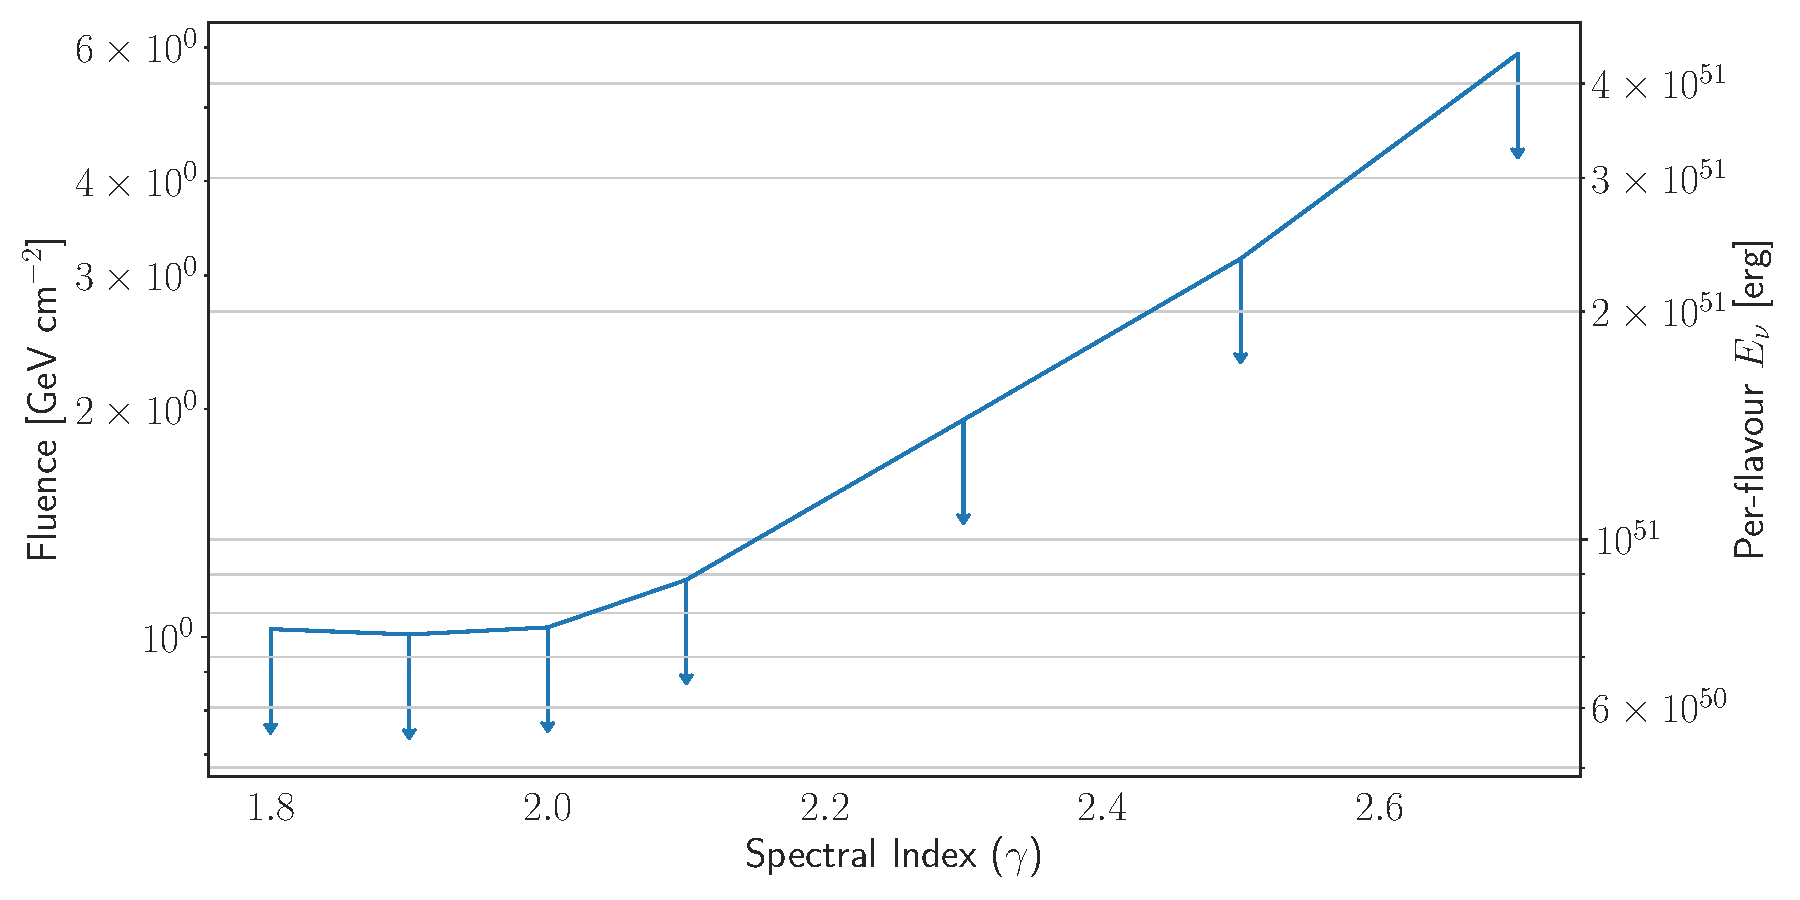
\includegraphics{results/at2018cow_limits}
	\caption{Limits on neutrino emission from AT2018cow, as a function of spectral index.}
	\label{fig:at2018cow_limits}
\end{figure}

The analysis of AT2018cow is the first example of a test for neutrino emission from FBOTs, a newly-identified class of transients. In the two years since discovery in 2018, there have been several theoretical studies considering possible neutrino emission from FBOTs in general, and AT2018cow in particular. Given that AT2018cow is by far the closest example of an FBOT, we can already consider the implications for the broader population emission, following the same procedure above.

\begin{figure}[!ht]
	\centering 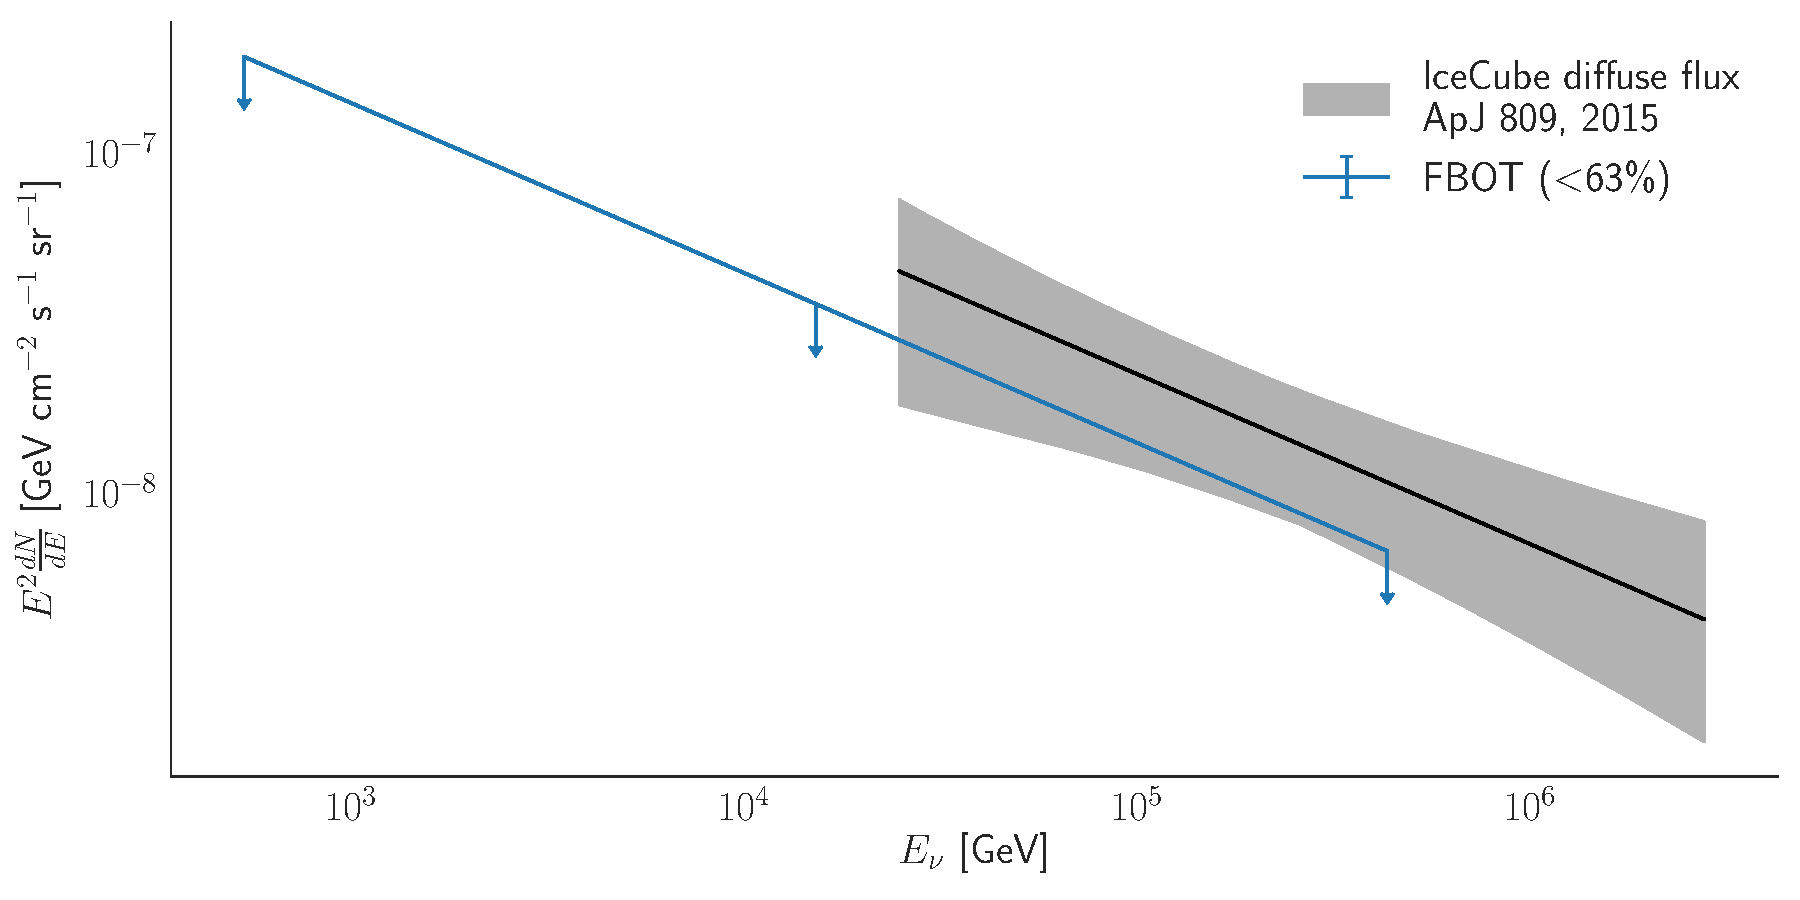
\includegraphics{results/fbot_limits}
	\caption{Limits on neutrino emission from from FBOTs, using the limits from AT2018cow under the assumption of neutrino standard candles.}
	\label{fig:fbot_limits}
\end{figure}